\documentclass[a4paper,12pt]{article} % тип документа

% report, book

% Рисунки
\usepackage{graphicx}
\usepackage{wrapfig}

\usepackage{hyperref}
\usepackage[rgb]{xcolor}
\hypersetup{				% Гиперссылки
    colorlinks=true,       	% false: ссылки в рамках
	urlcolor=blue          % на URL
}

%  Русский язык

\usepackage[T2A]{fontenc}			% кодировка
\usepackage[utf8]{inputenc}			% кодировка исходного текста
\usepackage[english,russian]{babel}	% локализация и переносы


% Математика
\usepackage{amsmath,amsfonts,amssymb,amsthm,mathtools} 


\usepackage{wasysym}

\author{Анна Назарчук Б02-109}
\title{1.4.1 Изучение экспериментальных погрешностей на примере физического маятника}
\date{}
\begin{document}
\maketitle
\section{Аннотация}
На примере измерения периода свободных колебаний физического
маятника познакомились с систематическими и случайными погрешностями, прямыми и косвенными измерениями; проверили справедливость формулы для периода колебаний физического маятника и определить значение ускорения свободного падения; убедились в справедливости теоремы Гюйгенса об обратимости
точек опоры и центра качания маятника; оценили погрешность прямых и косвенных измерений и конечного результата

\section{Теоретические сведения}
Физический маятник - твердое тело, совершающее колебания в поле силы тяжести, является свокупностью жестко связанных точечных масс. (рис. \ref{основа})

\begin{figure}[h!]
\begin{center}
\includegraphics[width=0.2\textwidth]{физмаятник}
\end{center}
\caption{Стержень как физический маятник} \label{основа}
\end{figure}

\subsection{Закон вращательного движения и момент инерции}
\begin{equation}\label{уравн-нью}
F = \frac{dp}{dt}
\end{equation}
\begin{equation}\label{уравн-нью}
Fr = \frac{d}{dt}(mr^2\omega) \quad \rightarrow \quad M = \frac{dL}{dt}
\end{equation}
$M$ - момент силы относительно оси вращения, $L = mr^2\omega\ = J\omega $ - момент импульса, $J = mr^2$ - момент инерции.
\begin{equation}
J = \sum_j m_jr_j^2
\end{equation}
Момент инерции тонкого стержня массой $m$ и длиной $l$, вращающегоя вокруг оси, проходящей через центр масс, равен: 
\begin{equation}
\label{инерциицм}
J_c=\frac{ml^2}{12}
\end{equation}
А момент инерции стержня с осью вращения на расстоянии $a$ от центра масс по теореме Гюйгенса-Штейнера:
\begin{equation}
\label{моментинерции}
J = \frac{ml^2}{12}+ma^2
\end{equation}
\section{Стержень как физический маятник}
\begin{equation}
\label{моменттяж}
M=-mgasin\varphi\approx-mga\varphi
\end{equation}
При малых отклонениях движение физического маятника будет иметь характер гармонических колебаний. Получим формулу для периода колебаний, используя аналогию с пружинным маятником, период которого равен $T=2\pi\sqrt{m/k}$. Роль массы играет момент инерции, роль коэффициента жесткости - коэффициент пропорцинальность между моментом силы и величиной отклонения.
\begin{equation}
\label{периодчерезинерции}
T=2\pi\sqrt{\frac{J}{mga}}
\end{equation} 
\begin{equation}
\label{период}
T=2\pi\sqrt{\frac{\frac{l^2}{12}+a^2}{ga}}
\end{equation}
Введем приведенную длину физического маятника:
\begin{equation}
\label{приведдлина}
l_\text{пр}=a+\frac{l^2}{12a}
\end{equation}
Теорема Гюйгенса: если стержень подвесить за центр качения (точка, отстоящая от точки опоры на $l_\text{пр}$ вдоль стержня), но период колебаний не изменится. 
\subsection{Гармонические колебания}
Получим формулу \ref{периодчерезинерции} через дифференциальное уравнение гармонических колебаний. Из \ref{основа} и \ref{моменттяж}:
\begin{equation}
\label{вращдиффур}
J\ddot{\varphi}+mga\varphi=0
\end{equation}
Решения уравнения будут вида:
\begin{equation}
\label{решениедиффура}
\varphi(t)=Asin(\Omega t+\alpha)
\end{equation}
где \(\Omega=\frac{2\pi}{T}=\sqrt{\frac{mga}{J}}\) - угловая частота колебаний, $A$ - угловая амплитуда, $\alpha$ - начальная фаза колебаний
\subsection{Затухание колебаний}
Если трение не слишком велико, колебания все еще могут быть описаны формулой \ref{решениедиффура}, но амплитуду колебаний следует счиать медленно убывающей функцией времени.
\[\gamma=\frac{|\Delta A|}{A}\]
$\gamma$ - декременант затухания (относительная убыль амплитуды за одно затухание), можно считать постоянным, поэтому:
\begin{equation}
\label{затухание}
A(t)=A_0e^{(-\gamma t)}
\end{equation} 

Добротность колебательной системы можно найти:
\begin{equation}
Q=\pi \frac{\tau_{\text{зат}}}{T}=\pi \frac{1/\gamma}{T}
\end{equation}
\subsection{Экспериментальная установка}
Тонкий стальной стержень длиной $l \backsim$ 1 м и массой $m \backsim$ 1 кг (точные
параметры определяются непосредственными измерениями) подвешивается на прикреплённой стене консоли с помощью небольшой призмы. Диаметр стержня много меньше его длины $d \backsim$ 12 мм $\ll l$. Небольшая призма
крепится на стержне винтом и острым основанием опирается на поверхность закреплённой на стене консоли. Острие ребра призмы образует ось
качания маятника.

\textbf{Установка А.}
Точку крепления можно перемещать вдоль стрежня, период колебания измеряется секундомером.


\section{Измерения и обработка результатов}
\subsection{Оборудование}
\textbf{Линейка}
\begin{equation}
\sigma_l = 0.5 \text{ мм}
\end{equation}

\textbf{Секундомер}
\begin{equation}
\sigma_t = 0.005  c
\end{equation}


\textbf{Максимальная относительная погрешность измерения периода колебаний маятника}
\begin{equation}
\varepsilon_{max} = 0.1 \%
\end{equation}

\textbf{Длина стержня}
\begin{equation}
l =100 \text{ см} 
\end{equation}

\textbf{Масса штанги}
\begin{equation}
m_{c} =870.3 \pm 0.1 
\end{equation}

\textbf{Масса призмы}
\begin{equation}
m_p =76.6 \pm 0.1 
\end{equation}

\textbf{Центр масс пустого стержня}
\begin{equation}
l_\text{ц} =50.1 
\end{equation}


\subsection{Оценка числа колебаний, требуемых для достижения нужной точности измерения}
Измерим период n  ($ n = 20$) колебаний  для экспериментального определения
случайной погрешности измерения времени с помощью секундомера.
\textbf{Положение призмы относительно центра масс}
\begin{equation}
l_{к} =75.3 \text{см} 
\end{equation}

\begin{table}
\caption{Измерение времени колебаний}
\begin{tabular}{|c|c|}
\hline 
№ опыта & t, c \\ 
\hline 
1 & 30.79 \\ 
\hline 
2 & 30.84 \\ 
\hline 
3 & 30.88 \\ 
\hline 
4 & 30.67 \\ 
\hline 
5 & 30.69 \\ 
\hline 
6 & 30.75 \\ 
\hline 
7 & 30.75 \\ 
\hline 
8 & 30.68 \\ 
\hline 
\hline
$\overline{t}$, c& 30.76 \\ 
\hline
$\sigma_t^\text{случ}$, c& 0.08 \\ 
\hline
$\sigma_t^\text{сист}$, c & 0.01 \\ 
\hline
$\sigma_t^\text{полн}$, c & 0.08 \\ 
\hline
\end{tabular} 
\end{table}
Откуда число колебаний, по которому следует измерять период, чтобы относительная погрешность измерений периода соответствовала точности измерений $\varepsilon_{max} = 0.1 \%$:  $n = 50$
\subsection{Опыт по измерению периода колебаний маятника по n полным колебаниям}
\begin{table}
\caption{Измерение периода колебаний маятника по n полным колебаниям (установка А) (без учета призмы)}
\begin{tabular}{|c|c|c|c|c|c|}
\hline 
№ опыта & $l_k$, см & a, см & $t_n$, с & $T$, с & $g$, м/$c^2$ \\ 
\hline 
1 & 75.3 & 25.2 & 76.85 & 1.54 & 9.74\\ 
\hline 
2 & 70.1 & 20 & 79.26 & 1.59 & 9.69\\ 
\hline 
3 & 63.4 & 13.3 & 87.46 & 1.75 & 9.80\\ 
\hline 
4 & 60.5 & 10.4 & 96.48 & 1.93 & 9.60\\ 
\hline 
5 & 57.5 & 7.4 & 110.78 & 2.22 & 9.65\\ 
\hline 
6 & 54.6 & 4.5 & 140.19 & 2.80 & 9.53\\ 
\hline 
7 & 87.3 & 37.2 & 77.76 & 1.56 & 9.73\\ 
\hline 
8 & 94.8 & 44.7 & 79.91 & 1.60 & 9.79\\ 
\hline 
9 & 72.1 & 22 & 77.85 & 1.56 & 9.75\\ 
\hline 
10 & 73.4 & 23.3 & 77.21 & 1.54 & 9.78\\ 
\hline 
11 & 73.6 & 23.5 & 77.28 & 1.55 & 9.74\\ 
\hline 
12 & 74.5 & 24.4 & 77.11 & 1.54 & 9.72\\ 
\hline 
\end{tabular} 
\end{table}



\begin{table}
\caption{Измерение периода колебаний маятника по n полным колебаниям (установка А) (с учетом призмы)}
\begin{tabular}{|c|c|c|c|c|c|c|}
\hline 
№ опыта & $l_k$, см & a, см & $x_\text{ц}$, см & $t_n$, с & $T$, с & $g$, м/$c^2$ \\ 
\hline 
1 & 75.30 & 25.20 & 23.10 & 76.85 & 1.54 & 9.76 \\ 
\hline
2 & 70.10 & 20.00 & 17.90 & 79.26 & 1.59 & 9.95\\ 
\hline
3 & 63.40 & 13.30 & 11.20 & 87.46 & 1.75 & 10.70\\ 
\hline
4 & 60.50 & 10.40 & 8.30 & 96.48 & 1.93 & 11.05\\ 
\hline
5 & 57.50 & 7.40 & 5.30 & 110.78 & 2.22 & 12.39\\ 
\hline
6 & 54.60 & 4.50 & 2.40 & 140.19 & 2.80 & 16.42\\ 
\hline
7 & 87.30 & 37.20 & 35.10 & 77.76 & 1.56 & 9.48\\ 
\hline
8 & 94.80 & 44.70 & 42.60 & 79.91 & 1.60 & 9.44\\ 
\hline
9 & 72.10 & 22.00 & 19.90 & 77.85 & 1.56 & 9.91\\ 
\hline
10 & 73.40 & 23.30 & 21.20 & 77.21 & 1.54 & 9.88\\ 
\hline
11 & 73.60 & 23.50 & 21.40 & 77.28 & 1.55 & 9.83\\
\hline
12 & 74.50 & 24.40 & 22.30 & 77.11 & 1.54 & 9.77\\ 
\hline

\end{tabular} 
\end{table}
\subsection{Обработка результатов}
Получим $g$ усредением полученных результатов (в оценке погрешности учитывается как случайная составляющая, так и систематическая:

$\overline{g_1} =9.97 \pm  0.16$ м/$c^2$ - с учетом призмы

$\overline{g_2} =9.73 \pm 0.16$ м/$c^2$ - без учета призмы
Дальнейшую обработку будем производить без учета призмы, так как относительная погрешность измерений больше 1\%, существенного вклада в точность результатов учет призмы не даст.
Построим график зависимости T(a). (рис. \ref{T(a)})
\begin{figure}[h!]
\begin{center}
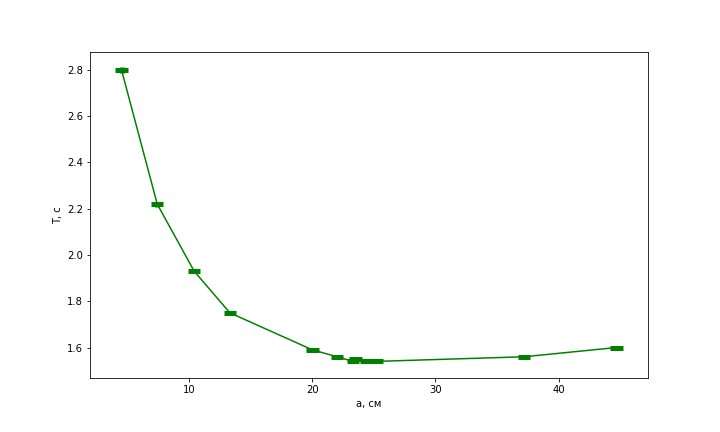
\includegraphics[width=\textwidth]{T(a)}
\end{center}
\caption{Зависимость периода колебаний от расстояния от точки крепления до центра масс} \label{T(a)}
\end{figure}

Найдем минимум с помощью графика (рис. \ref{T(a)+min} )
\begin{figure}[h!]
\begin{center}
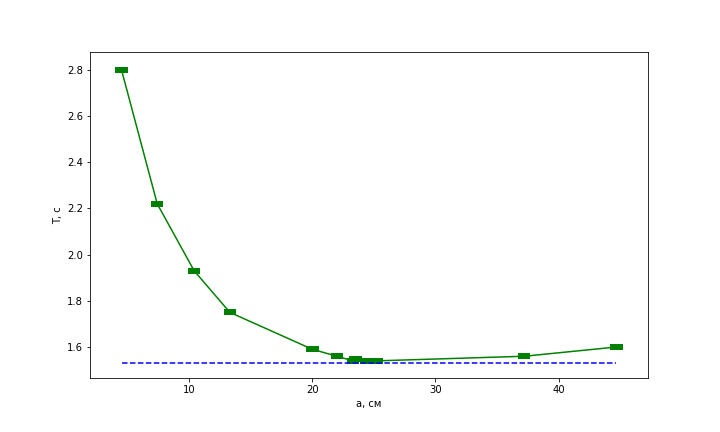
\includegraphics[width=\textwidth]{T(a)+min}
\end{center}
\caption{Зависимость периода колебаний от расстояния от точки крепления до центра масс с минимальным периодом} \label{T(a)+min}
\end{figure}

\begin{figure}[h!]
\begin{center}
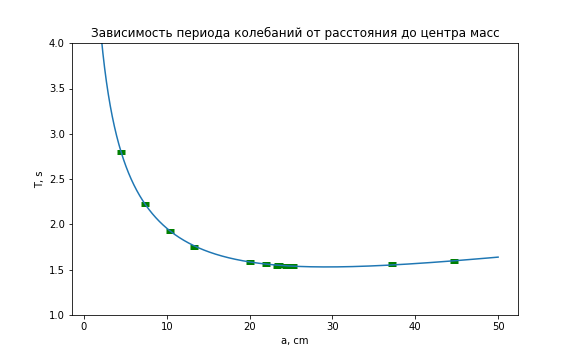
\includegraphics[width=\textwidth]{T(a)+fun}
\end{center}
\caption{Зависимость периода колебаний от расстояния от точки крепления до центра масс с аппроксимацией} \label{T(a)+fun}
\end{figure}

Обработка данных выдает зависимость периода от расстояния от точки крепления до центра масс, которая вместе с экспериментальными точками показана на рис. \ref{T(a)+fun}

$T_{min} = 1.53 $ с согласно графику, что согласуется с теоретическим расчетом ($T_{min} = 1.52$ с). В пределах округления период при измерении графически и аппроксимируя данные под функцию совпадает, но, конечно, измерение при помощи графика имеет существенно большую погрешность.

Построим график в координатах $u=\frac{T^2a}{4\pi^2}$, $v = a^2+\frac{l^2}{12}$ (рис. \ref{u(v)})
\begin{figure}[h!]
\begin{center}
\includegraphics[width=\textwidth]{u(v)}
\end{center}
\caption{График в координатах u(v)} \label{u(v)}
\end{figure}

Определим $g$ с помощью графика \ref{u(v)} МНК и оценим погрешность. В итоге получим, \[g=9.79 \pm 0.06 \text{ м/}c^2\]
Данным способом удалось получить меньшую погрешность и улучшить точность измерения.

Для одной из длин экспериментально сравним периоды колебаний физичекого маятника и математического с приведенной длиной нити (согласно формуле \ref{приведдлина}). 
$a= 25.2 $ см, $l_\text{пр}= 58.3$ см, $T_\text{ф}=1.54$ c, $T_\text{м}=1.54$ c, что согласуется с теорией.

Проверим справедливость теории Гюйгенса: точка опоры и центр качания маятника взаимно обратимы. 
$a_1= 25.2 $ см, $a_2= 58.3$ см, $T_1=1.54$ c, $T_2=1.54$ c, что согласуется с теорией.

\subsection{Затухающие колебания, вязкость воздуха}
Рассмотрим затухающие колебания. За $n=160$ колебаний, амплитуда уменьшилась в два раза. Поэтому
\[\gamma = \frac{\ln(2)}{nT}\]
\[Q=\pi\frac{\tau}{T}=\pi\frac{1/\gamma}{T}=\frac{\pi n}{\ln(2)}=725\]
Будем считать, что скорости маятника малы, амплитуды колебаний малы, сила сопротивления пропорциональна скорости.
\begin{equation}
F_c=-b\dot{x}
\end{equation}
\begin{equation}
m\dot{v}=-bv-mg\sin(\varphi)
\end{equation}
\begin{equation}
\ddot{\varphi}+\frac{b}{m}\dot{\varphi}+\frac{g}{l}\varphi=0
\end{equation}
\begin{equation}
\omega=\frac{g}{l}\gg \frac{b^2}{4m^2}
\end{equation}
\begin{equation}
\varphi(t)=\varphi_0e^{\frac{b}{2m}t}\cos(\omega t+\alpha)
\end{equation}
Рассмотрим амплитуду угла, которая изменяется согласно формуле \ref{затухание}
\begin{equation}
A=\varphi_0e^{\frac{b}{2m}t}
\end{equation}
Откуда можно было найти коэффициент пропорциональности в силе сопротивления, если знать массу:
\begin{equation}
\frac{b}{2m}=\gamma
\end{equation}
Согласно формуле Стокса:
\begin{equation}
b=6\pi r\mu
\end{equation}
Откуда динамическая вязкость воздуха:
\begin{equation}
\mu=\frac{b}{6\pi r}=\frac{2m\gamma}{6\pi r}
\end{equation}
Однако отсутствие данных для массы шарика не позволяет оценить вязкость воздуха.
\section{Выводы}
Проверена справедливость формулы для периода колебаний физического маятника и определено значение ускорения свободного падения; экспериментально подтверждена справедливости теоремы Гюйгенса об обратимости
точек опоры и центра качания маятника. 
Конечные резульаты измерения не отличаются большой точностью из-за наличия множества точек, в которых $a$ небольшое, поэтому относительная погрешность таких измерений высока. Также не совсем точно измерялось время колебаний, уменьшить эту погрешность можно с помощью многократных измерений, однако их количество должно быть невероятно велико для существенных улучшений.
\end{document}